\documentclass{amsart}
\usepackage{amssymb,latexsym,graphicx,verbatim}

\theoremstyle{definition}
\newtheorem{example}{Example}

\begin{document}

\title{A Brief Tutorial of the MATLAB PDE Toolbox}
\date{\today} % This shows up on the bottom of the page
\author[N.\, C. Ruderman]{Noah~C. Ruderman}
\author[I.\, F. Crosby]{Iain Crosby}
\author[T.\, A. Bakhtiyar]{Taha Bakhtiyar}
%\address{Department of Computer Science \\
%	   Brandeis University \\
% 	   Waltham, MA 02451}
\email[Noah~C. Ruderman]{noah3@brandeis.edu} % For multiple authors you may add the author's name as an optional argument
\email[Taha~A. Bakhtiyar]{tahaalib@brandeis.edu}
\email[Iain~F. Crosby]{icrosby@brandeis.edu}
\urladdr{https://sites.google.com/a/brandeis.edu/cs177-final-project/} %again, an optional argument exists for the name of the author

\begin{abstract}
For this project we explore some of applications of the PDE Toolbox in MATLAB 7.10.0. The work outlined here is ideal for someone who has a rudimentary knowledge of partial differential equations and has never used the PDE Toolbox before. First we briefly explain what a partial differential equation is and what partial differential equations the PDE Toolbox addresses. We then go on to explain applications of this toolbox and a brief descrption of the steps to solve a problem. To better aquaint the user with the toolbox, two examples are explained that nummerically solve a parabolic and elliptic differential equation.
\end{abstract}

\maketitle

\Large
\noindent
\textbf{What is a Partial Differential Equation?} \par
\normalsize
A differential equation is a mathematical equation in which an unknown function of several variables is related its derivaties of various orders. A partial differential equation (PDE) is similar to a differential equation in all ways except that the function of several variables is related to its partial derivatives of various orders with respect to those independent variables. Partial differential equations have applications in physics, engineering, as well as the applied sciences and are often used to model physical systems.
\par
\bigskip
\noindent
\Large
\textbf{What kind of PDEs can the PDE toolbox solve?} \par
\normalsize
There basic PDE solved by the PDE tool box is the equation
\begin{equation}
-\raisebox{.4ex}{$\bigtriangledown$} \cdot (c \raisebox{.4ex}{$\bigtriangledown$} u) + a u = f   \label{E:ellip} 
\end{equation}
We will express this equation as $\Omega$. Above is the elliptic equation. $\Omega$ is a bounded domain in the plane. $f, a, c,$ and the unknown $u$ are scalar complex valued functions defined on $\Omega$. The software can also handle the parabolic PDE
\begin{equation}
d \frac{\partial u}{\partial t} -\raisebox{.4ex}{$\bigtriangledown$} \cdot (c \raisebox{.4ex}{$\bigtriangledown$} u) + a u = f   \label{E:par}
\end{equation}
as well as the hyperbolic PDE
\begin{equation}
d \frac{\partial ^2 u}{\partial t^2} -\raisebox{.4ex}{$\bigtriangledown$} \cdot (c \raisebox{.4ex}{$\bigtriangledown$} u) + a u = f
\end{equation}
and finally the eigenvalue problem
\begin{equation}
-\raisebox{.4ex}{$\bigtriangledown$} \cdot (c \raisebox{.4ex}{$\bigtriangledown$} u) + a u = \lambda d u
\end{equation}
where $d$ is a complex valued function on $\Omega$, and $\lambda$ is an eigenvalue which will be determined by the solution to the equation. 

\par
\bigskip
\noindent
\Large
\textbf{In what areas is the PDE tool applicable?} \par
\normalsize
The PDEs listed above are used as mathematical models for a wide variety of problems and applications in engineering an the applied sciences. \par 
Some of the problems that can be solved and modeled by the elliptic and parabolic equations include:
\begin{itemize}
\item Heat transfer in solids
\item Diffusion
\item Electrostatics of dielectric and conductive media
\end{itemize}

The hyperbolic equation can be used for:
\begin{itemize}
\item Wave propagation in sound and electromagnetics
\item Transverse motion of membranes
\end{itemize}

The eigenvalue problems can model and solve:
\begin{itemize}
\item Finding the natural modes of vibrations in membranes and structural mechanics problems
\end{itemize}

\par
\bigskip
\noindent
\Large
\textbf{How do I use the PDE tool box to solve these problems?} \par
\normalsize
Using the PDE tool involves several steps:
\begin{itemize}
\item \emph{Defining a PDE problem}\\
To define a PDE problem we must know the general form of the PDE equation we will be using the solve the problem (parabolic, elliptic, hyperbolic, eigenvalue). We must also know the geometry of the problem that needs to be solved. For simple geometries, the built in functions of the PDE GUI will suffice. Simple geometries that can be drawn manually in the GUI include any intersection, union, or difference of shapes that include squares, rectangles, squares, ellipses, and irregularly shaped polygons. For more complex systems, an equation for the geometry of the shape can be entered through the command prompt in the form of an equation. Next, boundary conditions need to be specified for edges of the object and the edges of the subdomains. The boundary conditions come in the form of Dirichlet and Neumann boundary conditions. Dirichlet boundary conditions specify the value the solution must take on the boundary of the domain. A Neumann boundary condition specifies the value the derivative of a solution is to take on the boundary of the domain.
\item \emph{Solving the PDE} \\
The PDE tool box uses the Finite Element Method (FEM) for solving each of the PDE problems outlined here. The FEM involves creating a triangular mesh across the geometry of the object that the PDE will be solved for and solving at each of the verticies of the triangles. The FEM is a useful tool because often exact solutions are unattainable and often sufficiently accurate estimations suffice. The triangular mesh must be initialized and refined carefully. If the mesh is initialized but not refined or improved, some areas of the geometry may have less accurate estimations of the solution than desired. If the mesh is made to be too fine, MATLAB will spend time computing unnecessarily and slow the program down. Once the triangular mesh is in place in the correct orientation, MATLAB will solve the PDE instantly. 
\item \emph{Visualizing the results on a graph} \\
The results of the PDE solution can be visualized in several ways. The default option is to see a color grid with a color bar axis. Other options include the use of contour lines, a 3D plot, and animation mode. Animation mode plots the solution to the equation as a function over several different graphs depending on what time steps were specified in the GUI. 
\end{itemize}


\par
\bigskip
\noindent \Large We will cover the following examples:
\normalsize
\begin{enumerate} 
\item The heat flow problem \label{Heat Flow}
\item Conductive Media with an applied direct current \label{Electrostatics}
\end{enumerate}\vspace{12pt}

Note: For the benefit of the reader, images of GUI windows accessed from the main menu will be placed after their first reference so that the reader has a general idea of what using the GUI is like. To reduce redundancy, images of the windows referenced will not appear more than once.
\newpage

\begin{example}[The heat flow problem]

The basic form of the heat equation with a heat source is 
\begin{equation}
\frac{\partial u}{\partial t} = \alpha \left( \frac{\partial ^2 u}{\partial x^2} + \frac{\partial ^2 u}{\partial y^2} + \frac{\partial ^2 u}{\partial z^2}    \right) + q
\end{equation}
where $u$ is a function of $t,x, \text{ and } y$. In MATLAB this equation is parabolic and has the form of equation \eqref{E:par}. We can view this as 
\begin{equation}
d(t,x,y) \frac{\partial u}{\partial t} -\raisebox{.4ex}{$\bigtriangledown$} \cdot (c(t,x,y) \raisebox{.4ex}{$\bigtriangledown$} u) + a(t,x,y) u = f(t,x,y)
\end{equation}
On the main menu select \textbf{Options $\to$ Applications $\to$ Heat Transfer} to turn on the Heat Transfer Application mode. Our PDE retains the same form but becomes
\begin{equation}
\rho  C  u_t -\raisebox{.4ex}{$\bigtriangledown$} \cdot (k \raisebox{.4ex}{$\bigtriangledown$} u) = Q + h(u_{\text{ext}} - u)
\end{equation}
where $\rho$ is the density, $C$ is the heat capacity, $k$ is the coefficient of heat conduction, $Q$ is the heat source, $h$ is the convective heat transfer coefficient, and $u_{\text{ext}}$ is the external temperature.

We are going to model heat transfer across a plane sheet with the PDE Toolbox GUI. To bring up the PDE Toolbox GUI type \texttt{pdetool} in the MATLAB Command Window and press the enter key. 

\begin{figure}[ht]
   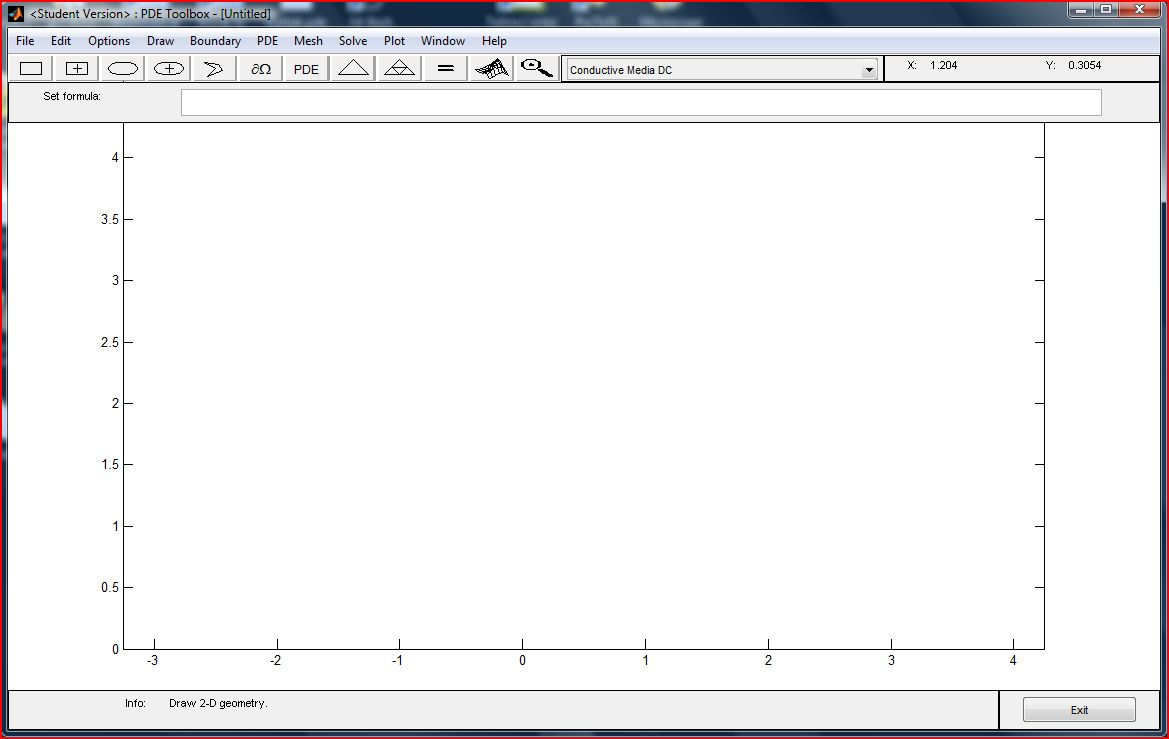
\includegraphics[height = 3 in]{pdetoolGUI}
   \caption{The pdetool GUI}
\end{figure}

To create the geometry of our plane sheet, click the icon on the toolbar that looks like a rectangle. Once selected, click with the right mouse button on the grid to draw a square of any size. Double click on the square to pull up the object dialog box. For the left and bottom coordinates, enter 0 for both values. Enter 2 for the height and 4 for the width. 

\begin{figure}[ht]
   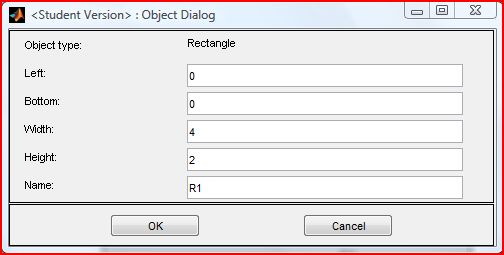
\includegraphics[height = 1.2 in]{ObjectDialogBoxRectangle}
   \caption{Object Dialog Box for a Rectangle}
\end{figure}

\pagebreak

The axes may need to be changed to visualize the entire object. To do so, on the main menu click  \textbf{Options $\to$ Axes Limits}, unclick the auto button for the y axis and adjust the y axis by changing it to [0 5]. Then on the main menu click \textbf{Options $\to$ Axes Equal}.

\begin{figure}[ht]
   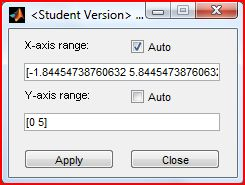
\includegraphics[height = 1.2 in]{AxesLimitsWindow}
   \caption{Axes Limits Window}
\end{figure}

\begin{figure}[ht]
   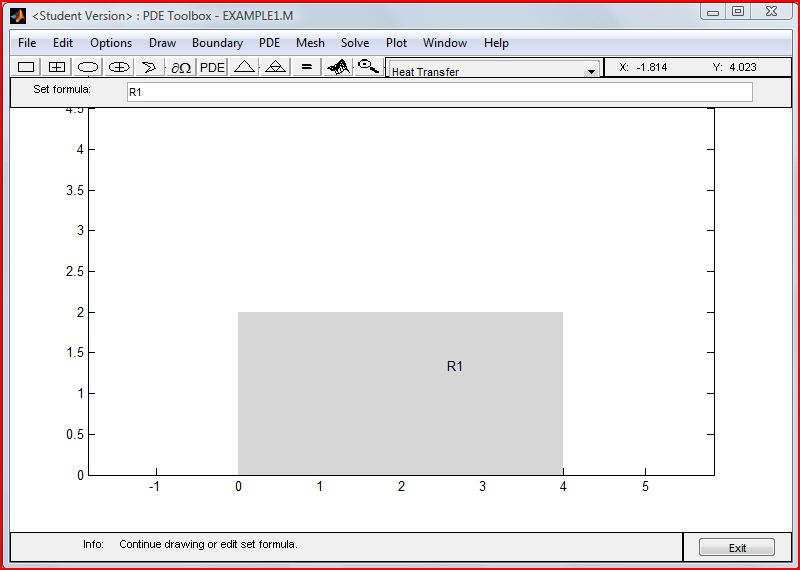
\includegraphics[height = 3 in]{DrawModeExample1}
   \caption{The Geometry of the Heat Transfer Problem}
\end{figure}
\pagebreak

Next, click the $\partial \Omega$ icon on the toolbar to enable boundary mode. Our boundary conditions are as follows
\begin{align*}
u_x(t,0,y) &= 1  	&&\text{left side} \\
u(t,4,y) &= 0 		&&\text{right side}  \\  
u_y(t,x,0) &= x 	&&\text{bottom}   \\
u(t,x,2) &= 0 		&&   \text{top} \\
u(0,x,y) &= 0 		&& \text{initial temperature}
\end{align*}
We see that the right and top sides are Dirichlet conditions, the left and bottom sides are Neumann conditions, and the last boundary condition is an initial condition. 

 In the Heat Transfer Application Mode, boundary conditions are of the form 
\begin{align*}
					&h \, u = r 	&& \text{Dirichlet} \\
n \, k \raisebox{.4ex}{$\bigtriangledown$} (u) {}+{} 	&q \, u = g 	&&\text{Neumann}
\end{align*}
where $h$ is the weight, $r$ is the temperature, $q$ is the heat transfer coefficient, and $g$ is the heat flux. We may interpret Dirichlet conditions as a heat source or heat sink at a boundary in which the heat source or sink is very large compared to the slab so we have no change in this boundary condition over time. We may interpret Neumann conditions as the flow of heat across a boundary in the direction perpendicular to the surface. In this equation, $n$ is a unit vector pointing in the direction perpendicular to the surface.

On the main menu click \textbf{PDE $\to$ PDE Specification.} On the left select the parabolic PDE option. Set $\rho = 1, C = 1, k = 1, Q = 2, h = 1, \text{ and } Text = 0$. 

\begin{figure}[ht]
   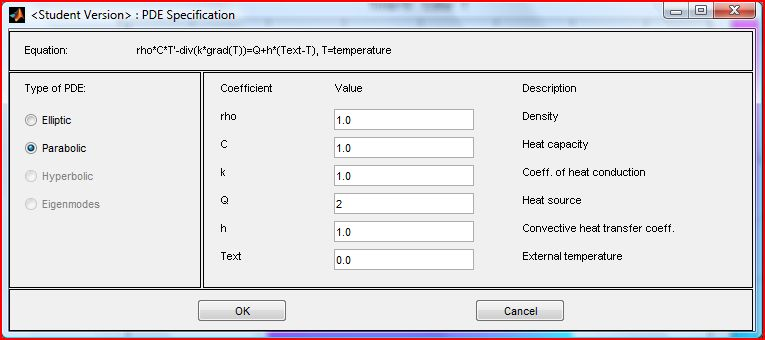
\includegraphics[height = 2 in]{PDESpecificationWindow}
   \caption{PDE Specification Window}
\end{figure}

To specify boundary conditions for the sides of the slab, double click on one side or click on one side and then from the main menu select  \textbf{Boundary~$\to$~Specify Boundary Conditions.} For the top and right side, select Dirichlet and change $h$ to 1 and $r$ to 0. For the left side, select Neumann conditions and set $g = 1$ and $q = 0$. For the bottom side, select Neumann conditions and set $g = x$ and $q = 0$. 

\begin{figure}[ht]
   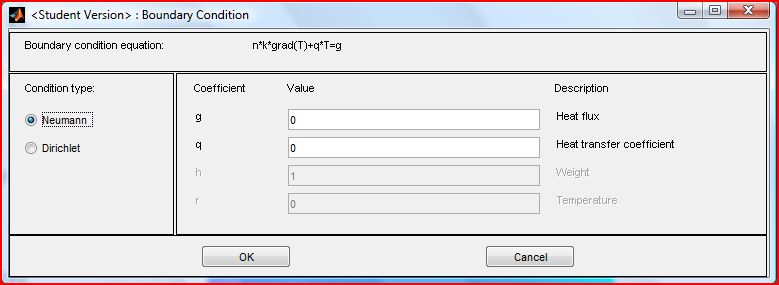
\includegraphics[height = 1.5 in]{BoundaryConditionWindow}
   \caption{Boundary Condition Window}
\end{figure}

\pagebreak

To specify the initial conditions, from the main menu select \textbf{Solve $\to$ Parameters.} Enter 0 for $u(t_0)$ for our initial temerature. This is also where we can specify the times that the PDE will be solved for. Input  linspace(0,5,10) to specify the times solved for.

\begin{figure}[ht]
   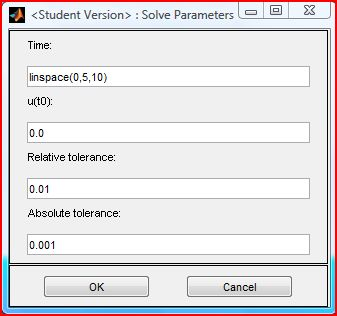
\includegraphics[height = 2 in]{SolveParametersWindow}
   \caption{The Solve Parameters window}
\end{figure}

To initialize the mesh press the $\triangle$ icon on the toolbar or use the main menu by selecting \textbf{Mesh $\to$ Initialize Mesh}. For greater accuracy, the mesh can be refined by clicking the icon with 4 triangles or clicking \textbf{Mesh $\to$ Refine Mesh.} This increases the number of points that the PDE is solved numerically reducing the error but increasing the calculation time. Generally mesh should only be refined only if more accuracy is needed. Whenever the mesh is refined, the mesh should be jiggled. You can jiggle the mesh by selecting \textbf{Mesh $\to$ Jiggle Mesh} from the main menu.

\begin{figure}[h]
   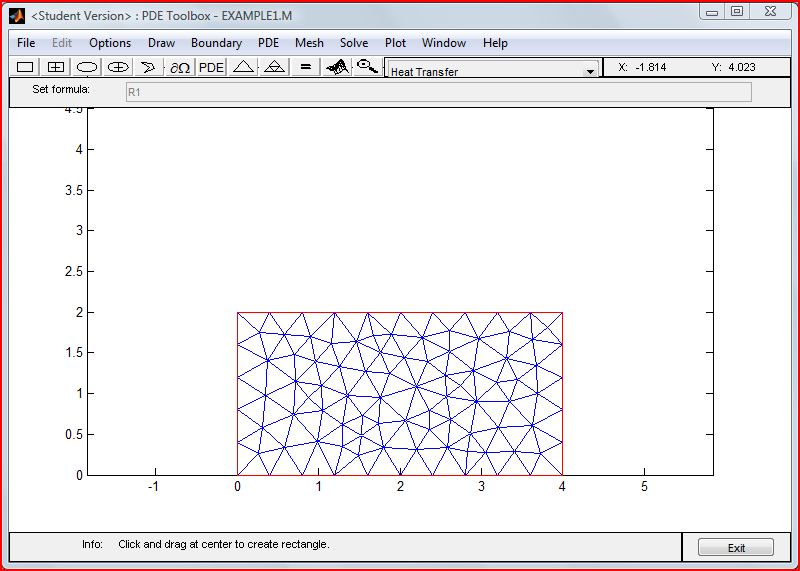
\includegraphics[height = 3 in]{MeshModeExample1}
   \caption{A single triangle mesh}
\end{figure}

\pagebreak

To solve the PDE simply click $=$ icon on the toolbar. Alternatively use the main menu by clicking \textbf{Solve $\to$ Solve PDE.} The default solution is a colorbar of the system at the time of the last solution.

\begin{figure}[h]
   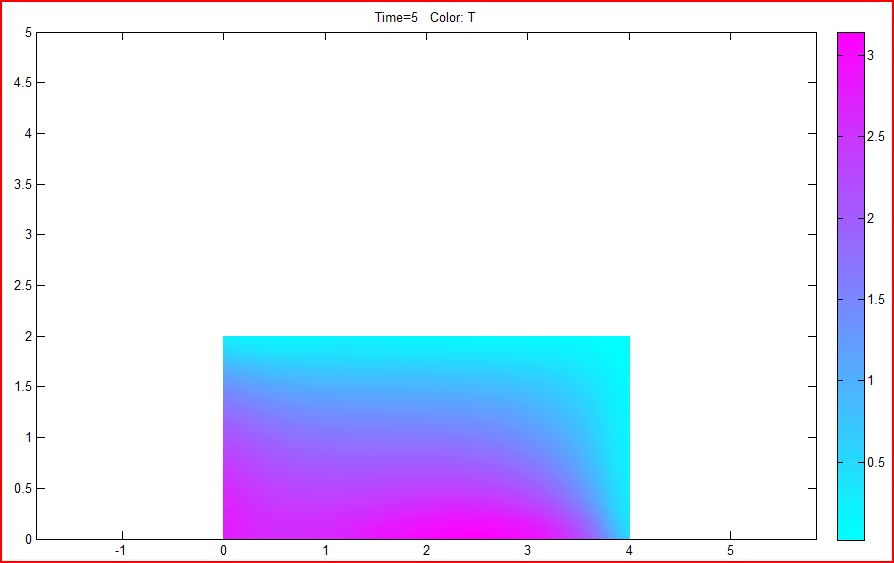
\includegraphics[height = 3 in]{Example1FinalGraph}
   \caption{The PDE solved for the last time step}
\end{figure} 

To see alternate visualizations, from the main menu select \textbf{Plot $\to$ Parameters.} On the left the type of plot can be specified. Select Height (3-D plot) option and the Animation option. Now plot the solution to see the animation.

\begin{figure}[h]
   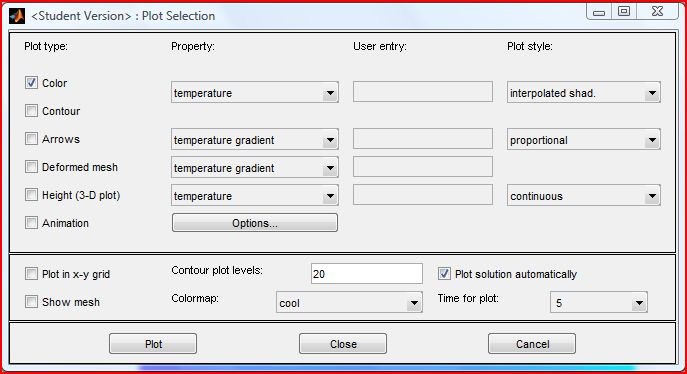
\includegraphics[height = 2.5 in]{PlotSelectionWindow}
   \caption{The Plot Selection window}
\end{figure}
\end{example}

We can save our work by clicking on \textbf{File $\to$ Save} from the main menu. If we choose to open this file throught the PDE Toolbox GUI, our previous work appears back on the screen as it was at the time it was saved. Opening the file from the editor window in MATLAB opens the script file of our work.

\phantom{newspace} \newpage

\begin{example}[Conductive Media DC] \hfill \\
\indent
In this next example we will be modeling the potential and current flow on a metal sheet with several smaller circular metal sheets placed on top but each held at different voltages.  We will make one of the circles have a negative potential, while the other two will be positive.  To do this we will be using the Poisson equation. To derive this, we start with the knowledge that 
\begin{gather}
J = \sigma E         \label{E:J} \\
\raisebox{.4ex}{$\bigtriangledown$} \cdot J = q        \label{E:Q} \\
E = -\raisebox{.4ex}{$\bigtriangledown$} V           \label{E:E}
\end{gather}
Note: $\sigma$ is the conductivity, $J$ is the volume current, $E$ is the electric field, $V$ is the electric potential, and $q$ is our current source. We substitute the relation for $J$ from equation \eqref{E:J} into equaiton \eqref{E:Q} to get
\[
\raisebox{.4ex}{$\bigtriangledown$} \cdot \sigma E = q
\]
Now we sub in $E$ from equation \eqref{E:E} to get
\[
\raisebox{.4ex}{$\bigtriangledown$} \cdot \sigma (-\raisebox{.4ex}{$\bigtriangledown$} V) = q
\]
which is equal to 
\begin{equation}
-\raisebox{.4ex}{$\bigtriangledown$} \cdot \left( \sigma \raisebox{.4ex}{$\bigtriangledown$} V \right)= q     \label{E:Poisson}
\end{equation}
which is the Poisson equation. We can see that this is in the form of an elliptic equation in which $V$ is our solution, $c = \sigma, a = 0, \text{ and } f = q$.

First we will create the geometry of our system. To specify our geometry we create four shapes. First create a rectangle by clicking on the rectangle icon on the toolbar and draw any sized rectangle. Double click on the rectangle to pull up the Object Dialog and enter the value 0 for the left and bottom coordinates. Make the width 2 and the height 4. On the main menu, go to \textbf{Options $\to$ Axes Limits.} Enter the vector [0 5] for the y axis limits. On the main menu select \textbf{Options $\to$ Axes Equal.}

Next click the circular icon on the toolbar and draw a circle by clicking the right mouse button and dragging. Repeat this three times. Now double click on each circle to open the object dialog box and change the parameters. Make the object designated C1 to have a center at (1, 3.5) with a radius of 0.4. Make the object designated C2 to have a center at (1, 2) with a raidus of 0.4. Make the object designated C3 to have a center at (1, 0.5) with a raidus of 0.4. Next, go to the set formula that is on the top of the GUI but below the toolbar to SQ1 - (C1+C2+C3).

\begin{figure}[ht]
   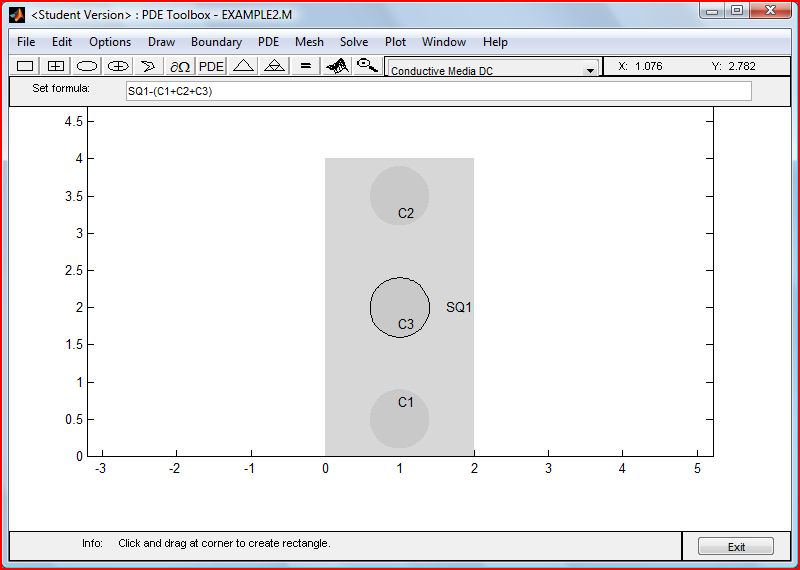
\includegraphics[height = 3 in]{DrawModeExample2}
   \caption{The Geometry of the Conductive Media DC Problem} \label{F:picture}
\end{figure}

Now click the $\partial \Omega$ symbol in the toolbar to enable boundary mode. 
The boundary conditions are as follows:
\begin{align*}
&V = 1              	&& \text{on the top circular conductor} \\
&V = 2              	&&\text{on the middle circular conductor} \\
&V = -1            	&&\text{on the bottom circular conductor} \\
&\frac{dV}{dn} = 0 	&&\text{on the boundaries of the rectangular sheet} 
\end{align*}
We can see that the first three boundary conditions are Dirichlet conditions and the last boundary condition is a Neumann condition. In the Conductive Media DC Application Mode, boundary conditions are of the form 
\begin{align*}
					&hV = r 	&& \text{Dirichlet} \\
n\sigma \raisebox{.4ex}{$\bigtriangledown$} (V) {}+{} 	&q V = g 	&&\text{Neumann}
\end{align*}
where $h$ is the weight, $r$ is the electric potential, $n$ is a unit vector pointing perpendicular to the edge, $g$ is the current source, and $q$ is the film conductance.

To select boundary conditions, click on an edge and on the main menu click \textbf{Boundary $\to$ Specify Boundary Conditions.} On the edges of the the square (select multiple edges by holding shift and selecting each edge to include), select Neumann boundary conditions and set $g = q = 0$. For each circular conductor, select all edges and then select Dirichlet boundary conditions. Set $h = 1$ and set $r$ to the appropriate potential. 

Open the PDE specification box by selecting \textbf{PDE $\to$ PDE Specification} on the main menu. We the same PDE as modeled by equation \eqref{E:Poisson}. Set $\sigma = 1$ and $q = 0$. 

Next initialize the mesh by selecting \textbf{Mesh $\to$ Initialize Mesh} from the main menu. Now select \textbf{Mesh $\to$ Refine Mesh} and jiggle the mesh once by selecting \textbf{Mesh $\to$ Jiggle Mesh.}

\begin{figure}[ht]
   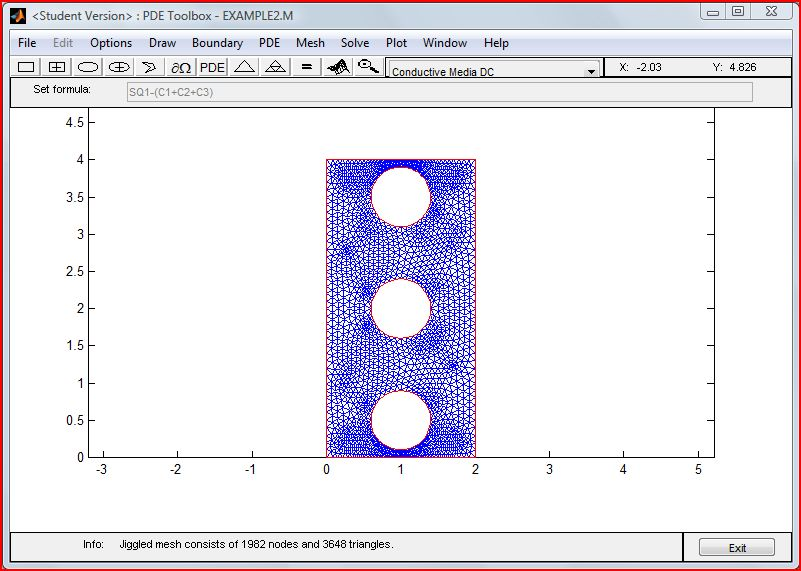
\includegraphics[height = 3 in]{MeshModeExample2}
   \caption{Mesh mode after two mesh refinements and jiggling}
\end{figure}

\newpage

Now to specify the graph we will plot, from the main menu select \textbf{Plot $\to$ Parameters.} On the left check the Countour and Arrow boxes under plot type. Close the box.

To solve the equation, click the $=$ button icon in the toolbar and the solution is plotted automatically.

\begin{figure}[ht]
   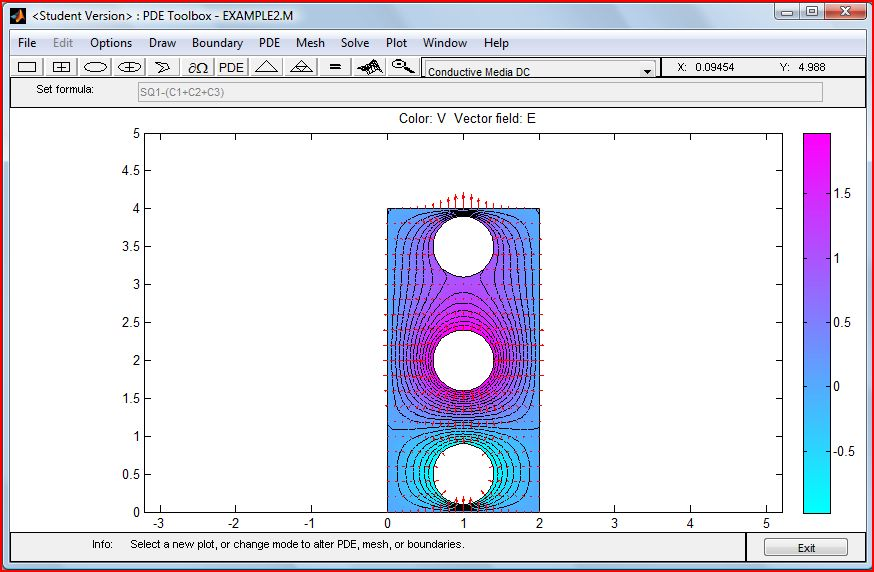
\includegraphics[height = 3 in]{Example2FinalGraph}
   \caption{The PDE solved for the last time step}
\end{figure}

\end{example}

\begin{thebibliography}{9}
   \bibitem{pH11}
   Peter Howard
   "Partial Differential Equations in MATLAB 7.0."
   Web.
   4 May 2011

   \bibitem{mW11}
   MathWorks, ed.
   MATLAB PDE User Guide.
   Natick, MA:
   Mathworks, 2011.
   Print.

   \bibitem{wP11}
   Wikipedia contributors.
   "Partial differential equation."
   Wikipedia, The Free Encyclopedia.
   Wikipedia, The Free Encyclopedia, 20 Apr. 2011.
   Web.
   5 May. 2011
   \verb+http://en.wikipedia.org/w/index.php?title=Partial_differential_equation&oldid=425056169+
\end{thebibliography}

\end{document}